%! TEX root = **/000-main.tex
% vim: spell spelllang=en:
\chapter{Appendix}

\section{Paired t-test asin vs asin norm}

\begin{figure}[H]
    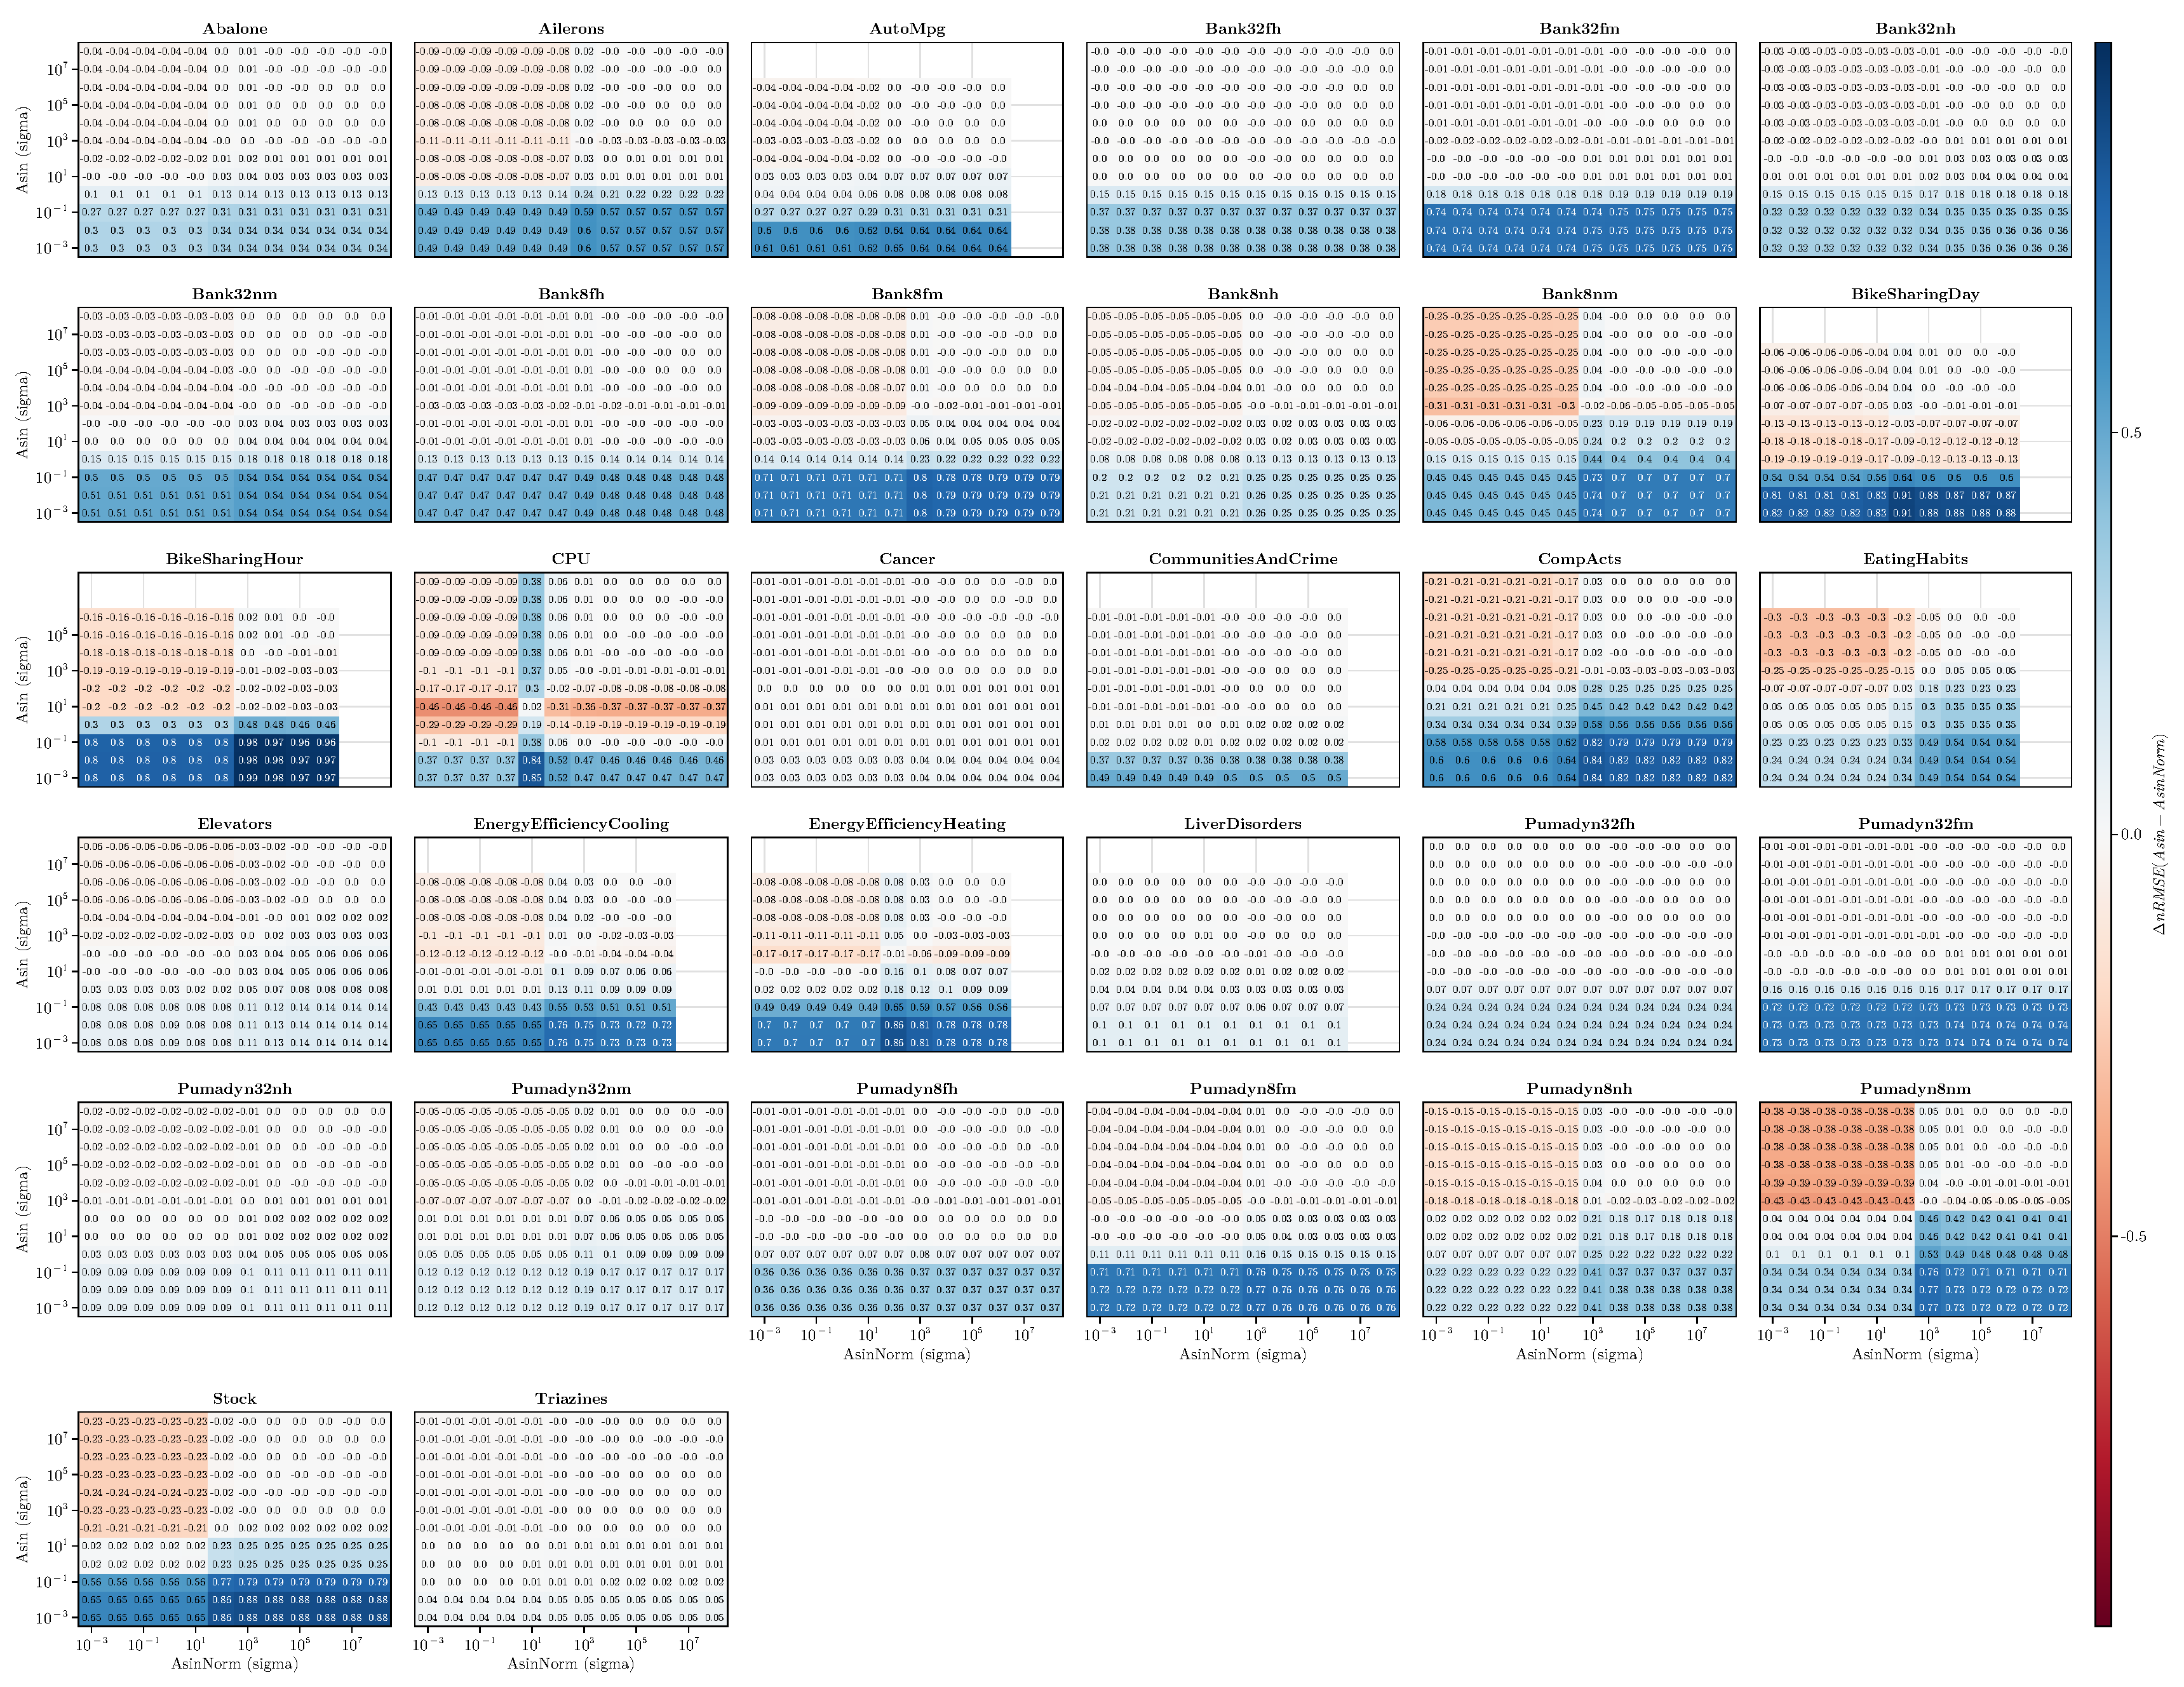
\includegraphics[width=0.9\textwidth]{plots/heatmaps_asin_asinnorm}
    \caption{Difference between nRMSE of RBF and normalized arc-sine kernels ($\alpha=0.001$)}
    \label{fig:paired-ttest-asin-asinnorm-diff}
\end{figure}

\section{Additional plots}

% NOTE: this is without scaling sigma
\begin{figure}[H]
    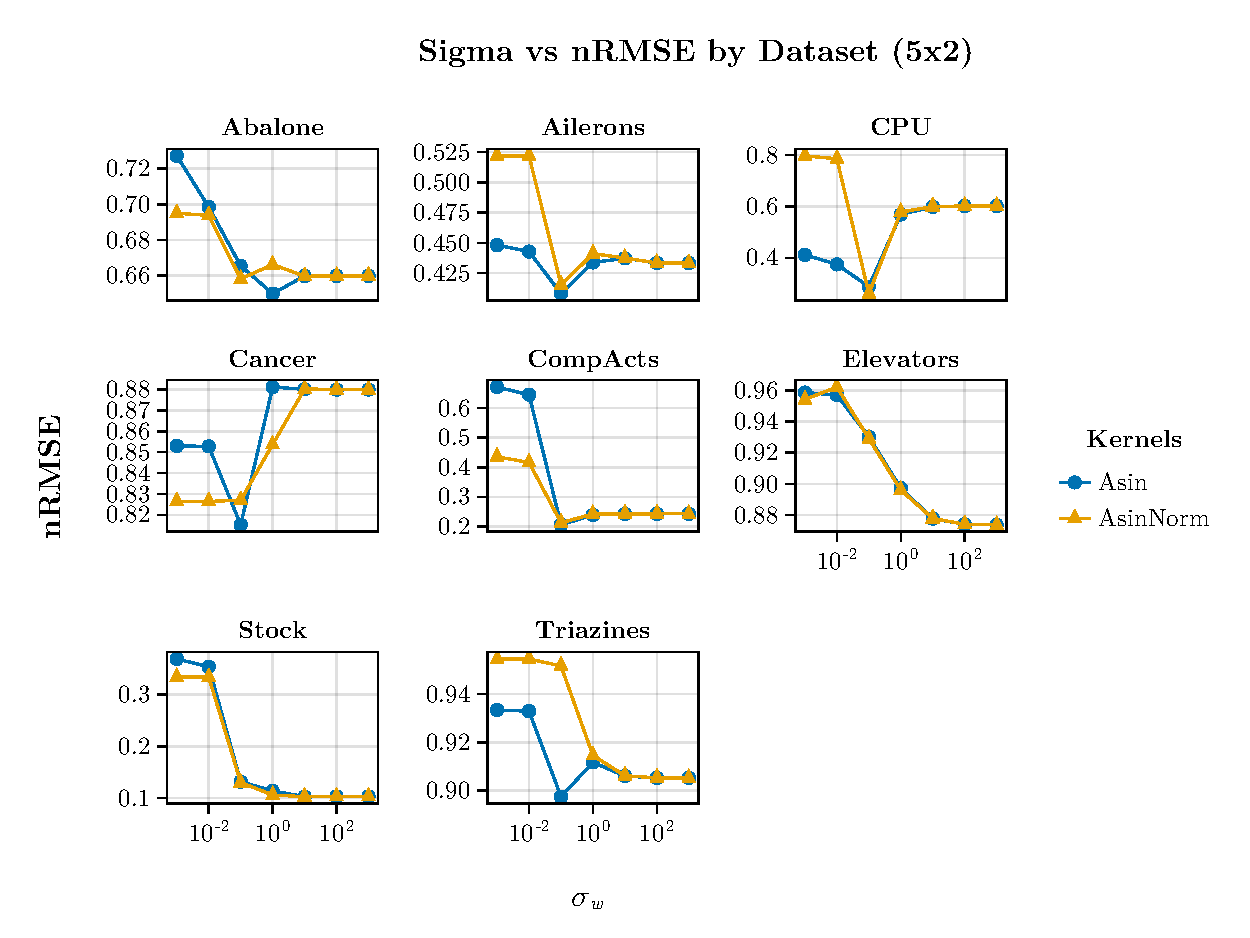
\includegraphics{plots/nRMSE_frenay}
    \caption{nRMSE results on datasets from \cite{frenayParameterinsensitiveKernelExtreme2011}}
\end{figure}

% WARN: these don't have all values of epsilon in our grid
\begin{figure}[H]
    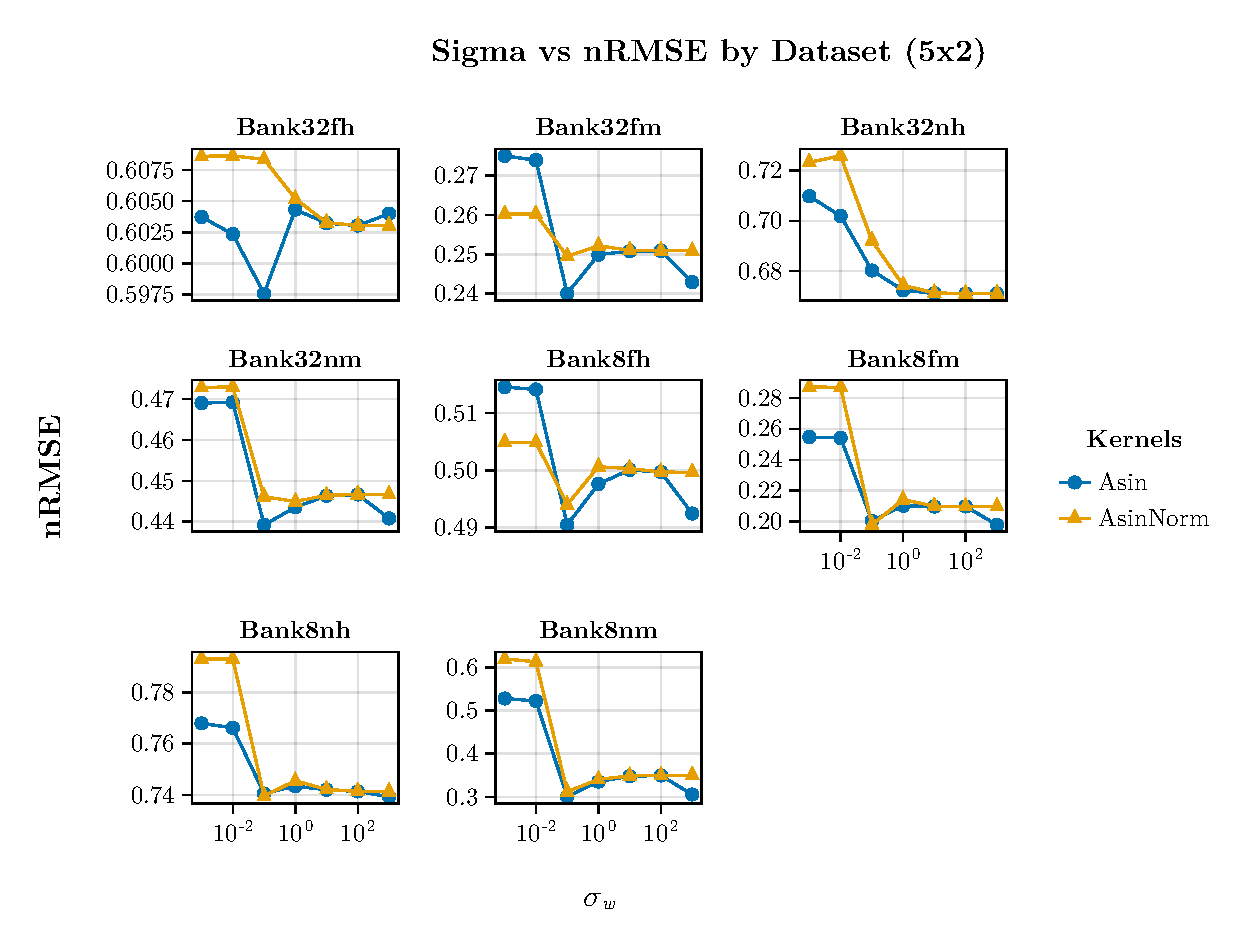
\includegraphics{plots/nRMSE_bank}
    \caption{nRMSE results on Delve Bank dataset}
\end{figure}

% WARN: these don't have all values of epsilon in our grid
\begin{figure}[H]
    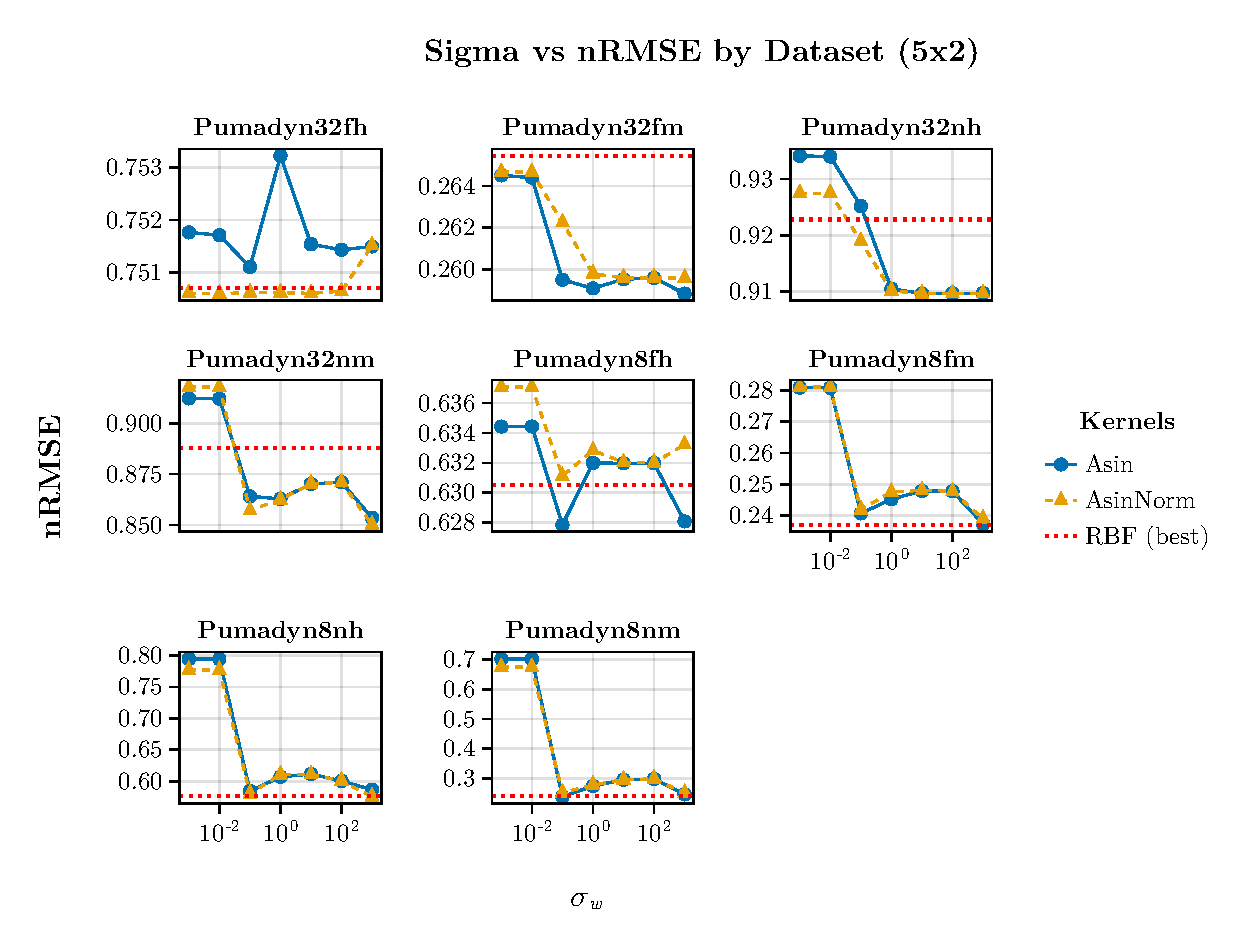
\includegraphics{plots/nRMSE_pumadyn}
    \caption{nRMSE results on Delve PumaDyn dataset}
\end{figure}

\begin{figure}[H]
    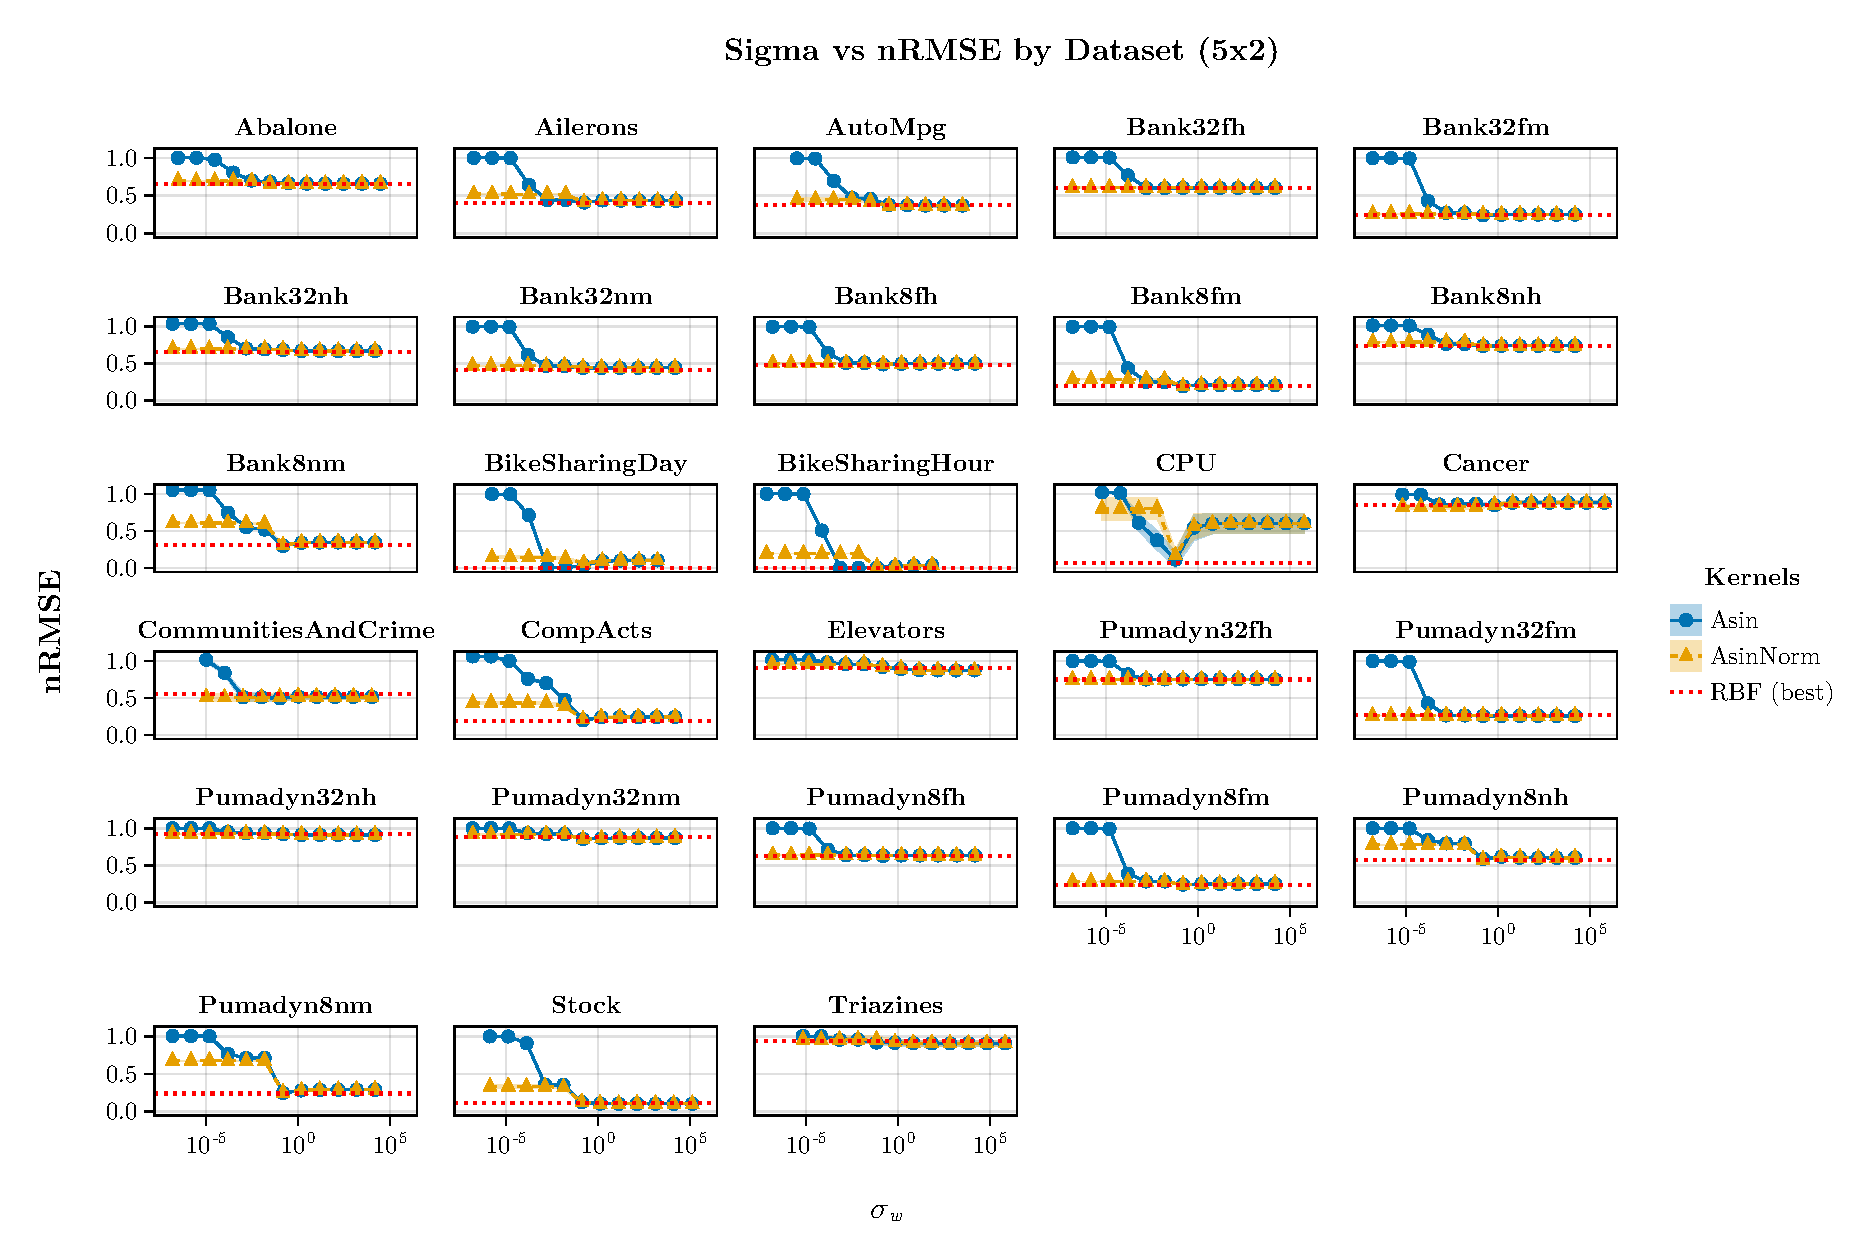
\includegraphics{plots/nRMSE_all_scaled}
    \caption{nRMSE results on Regression datasets with $\sigma_w$ scaled}
\end{figure}

\begin{figure}[H]
    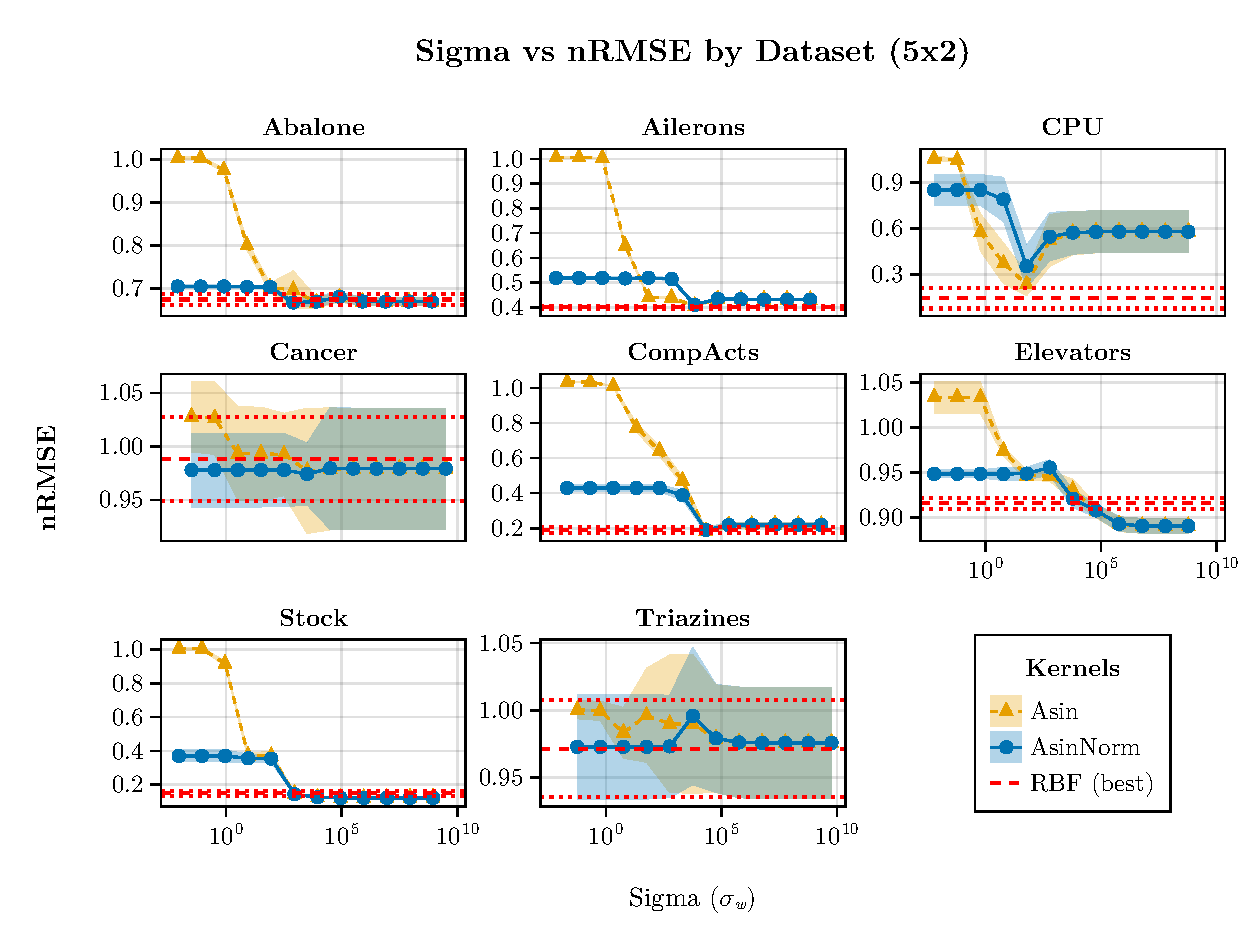
\includegraphics{plots/nRMSE_frenay_scaled}
    \caption{nRMSE results on Frenay datasets with $\sigma_w$ scaled}
\end{figure}

\subsection{3D kernels}

% 3d version
\begin{figure}
    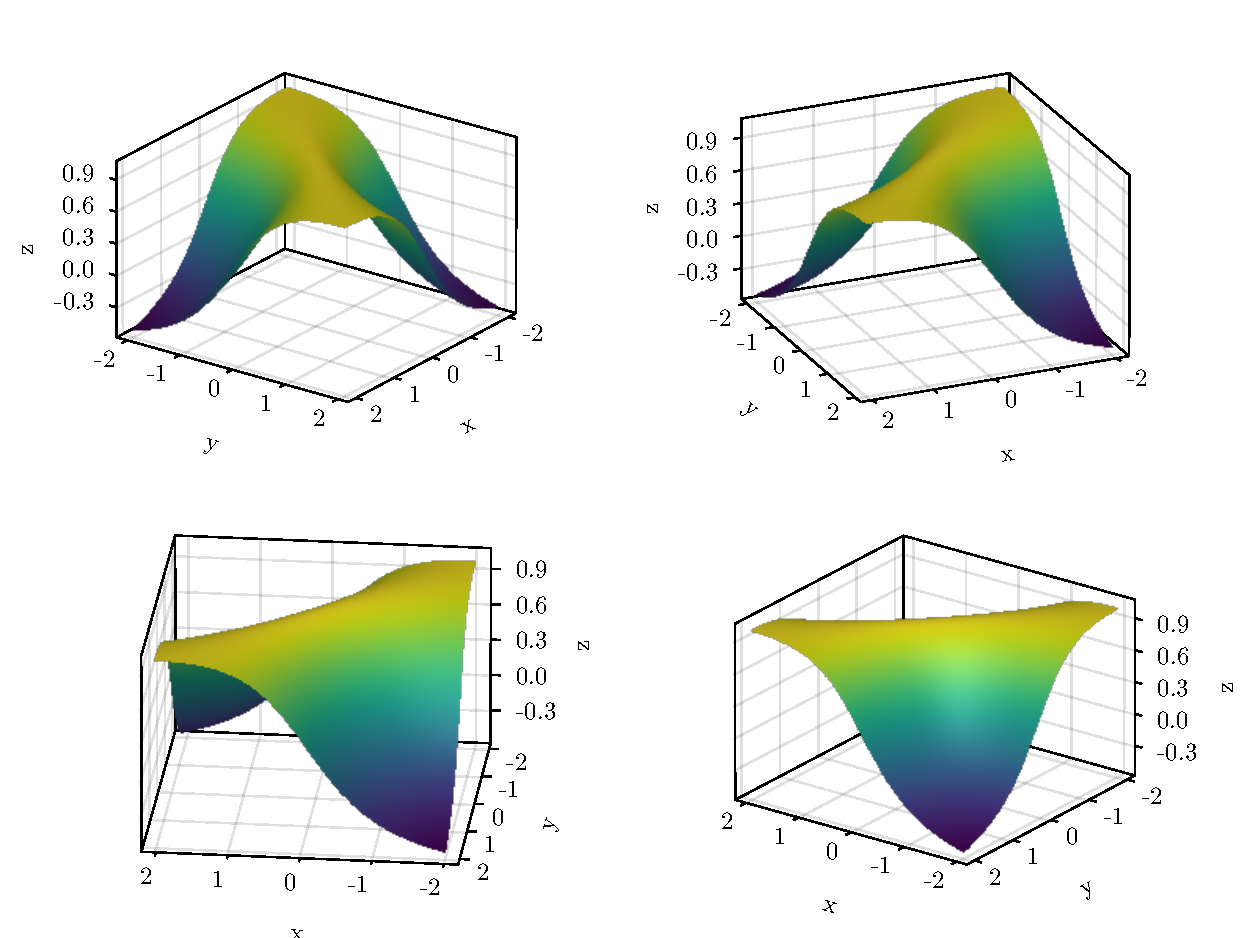
\includegraphics{plots/kernel_asin_3d_sig1}
    \caption{asin kernel with $\sigma_w=1$}
\end{figure}

\begin{figure}
    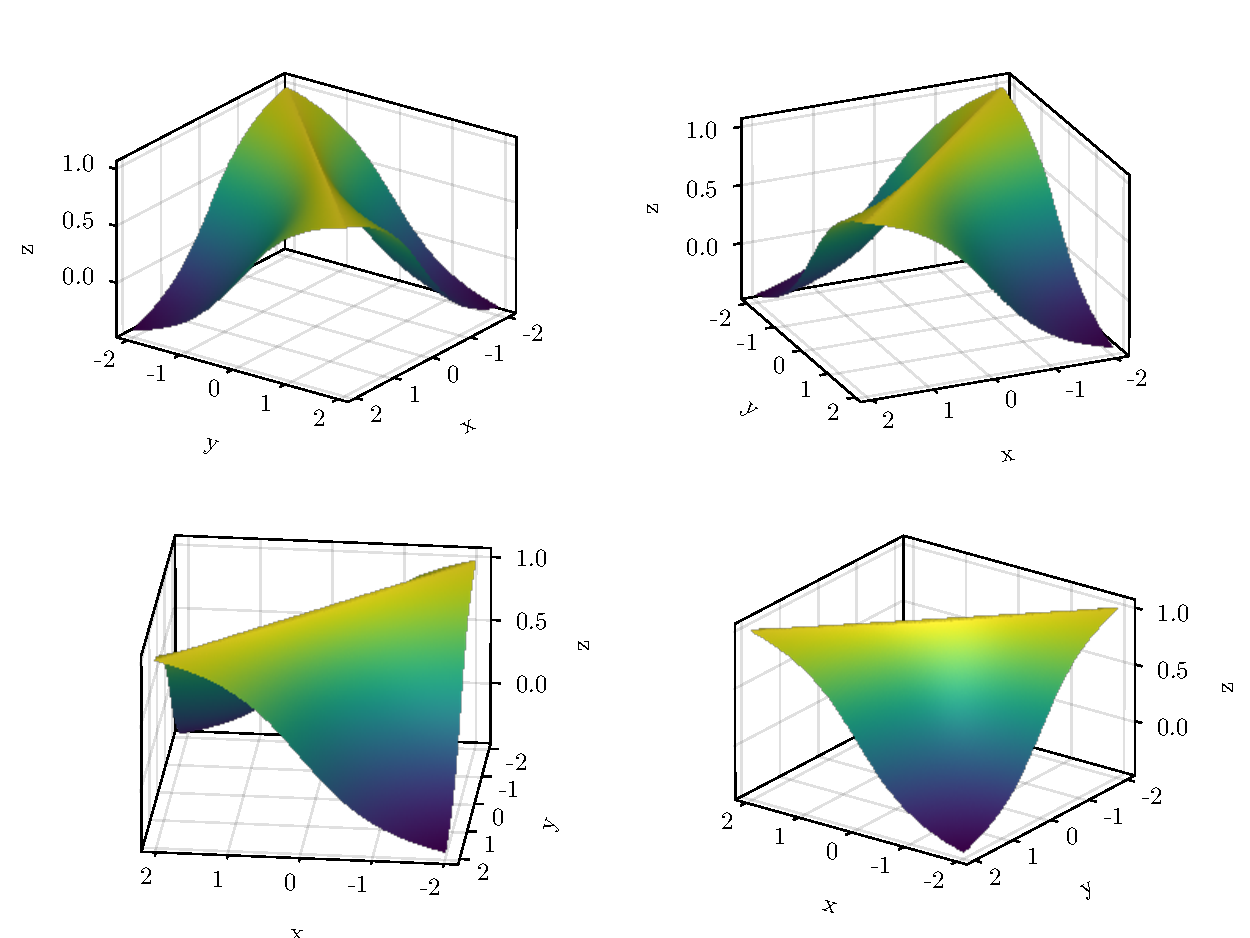
\includegraphics{plots/kernel_asin_3d_sig1000}
    \caption{asin kernel with $\sigma_w=1\,000$}
\end{figure}


% The acos ones are not very interesting with one dimensional vectors
\begin{figure}
    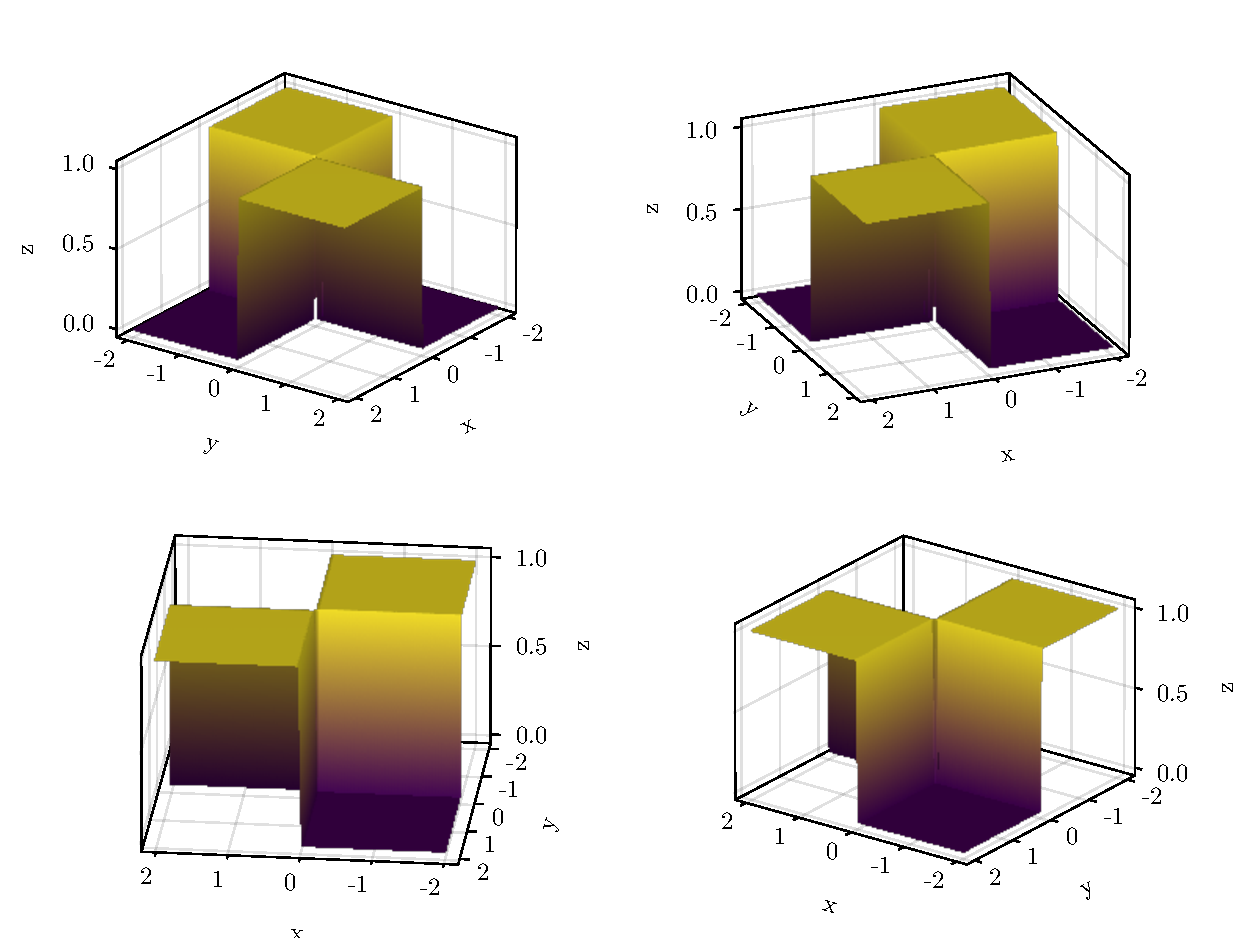
\includegraphics{plots/kernel_acos0_3d}
    \caption{acos kernel $n=0$}
    \label{fig:kernel_acos0_3d}
\end{figure}

\begin{figure}
    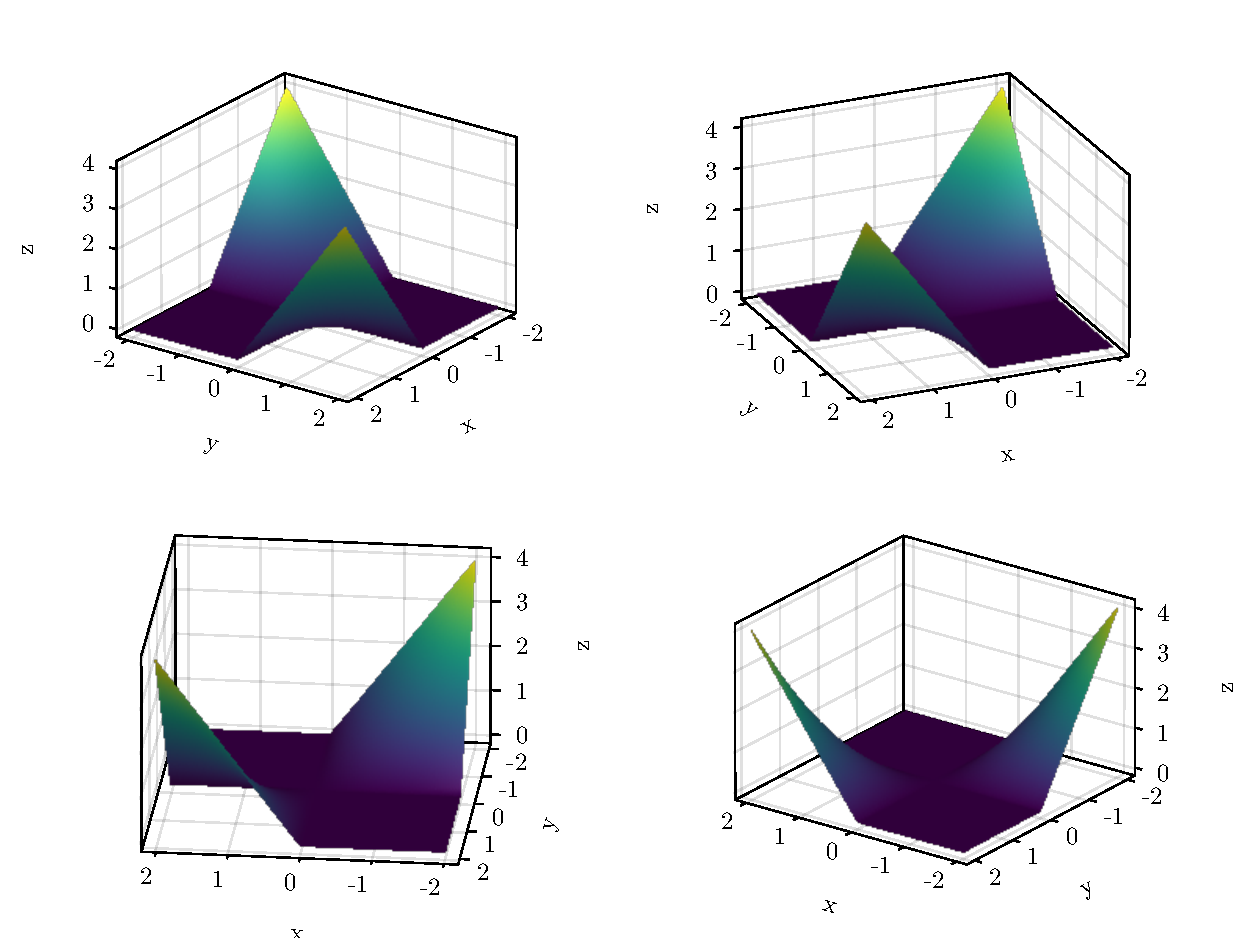
\includegraphics{plots/kernel_acos1_3d}
    \caption{acos kernel $n=1$}
\end{figure}

\begin{figure}
    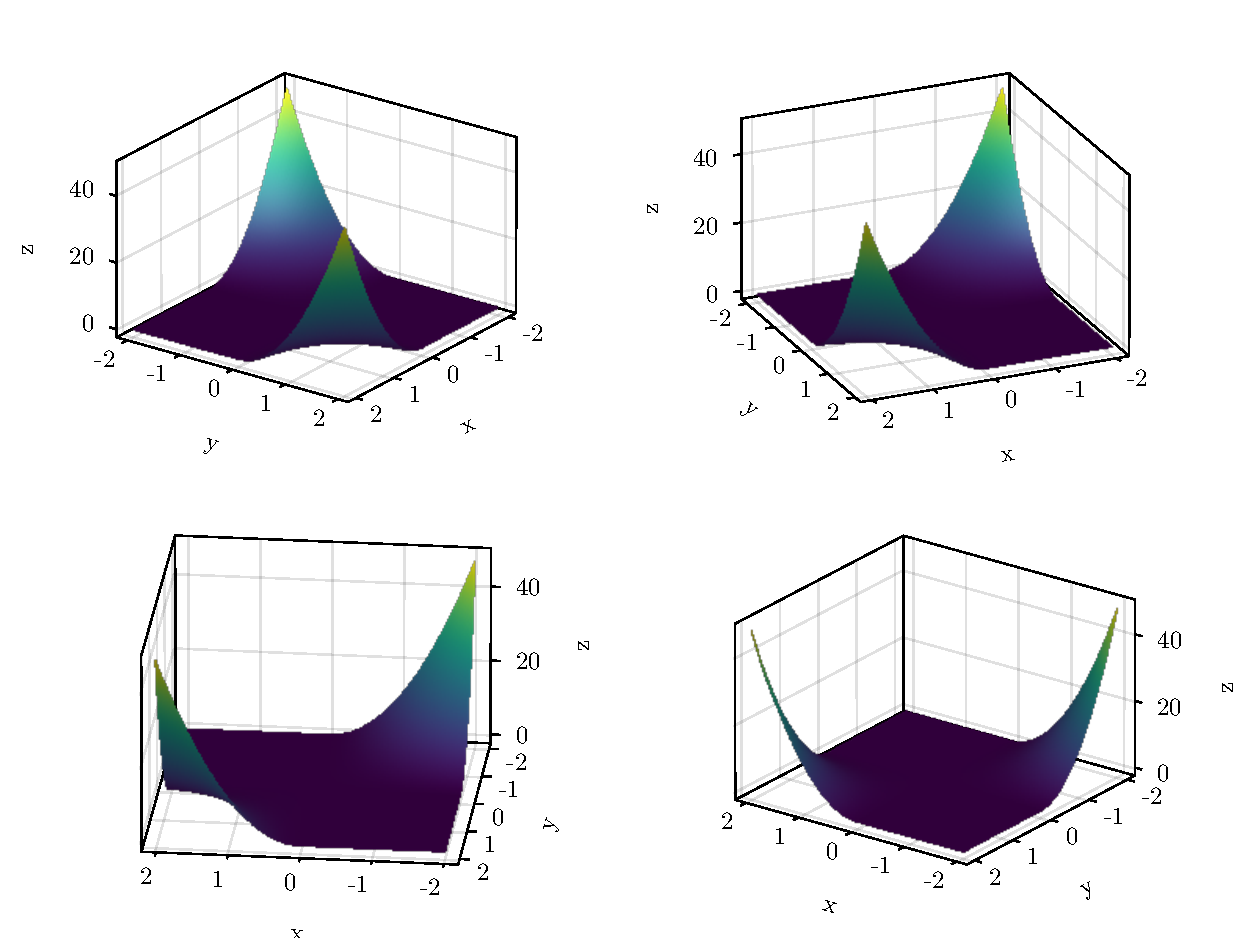
\includegraphics{plots/kernel_acos2_3d}
    \caption{acos kernel $n=2$}
\end{figure}

% TODO: remove
\section{Kernels}
\subsection{Arc sine kernel}

\textcite{frenayParameterinsensitiveKernelExtreme2011,williamsComputationInfiniteNeural1998}:


\begin{equation}
    \erf(x) = \frac{2}{\sqrt{\pi}} \int_0^x e^{-t^2} \,dt
\end{equation}

% TODO: Put integral from William
% \begin{equation}\label{eq:asin_integral}
% \begin{equation}

\begin{equation}
    V_{\erf}\left(\x,\,\x'\right) =
    \frac{1}{(2\pi)^{\frac{d+1}{2}} |\boldsymbol \Sigma|^{\frac{1}{2}}}
    \int
    \erf \left(\bu ^T \tilde \x \right)
    \erf \left(\bu ^T \tilde \x '\right)
    \exp \left(
    -\frac{1}{2} \bu ^T \boldsymbol \Sigma^{-1} \bu
    \right)
    \,d\boldsymbol u
\end{equation}

Appropriately scaled, the graph of this function is very similar to the
\texttt{tanh} function, which is more commonly used in the neural networks'
literature \cite{williamsComputationInfiniteNeural1998}.

\begin{equation}
    k(\x,\,\z \mid p \to + \infty)  = \frac{2}{\pi}
    \arcsin \frac{1 + \left\langle \x,\,\z \right\rangle}{\sqrt{
            \left(
            \frac{1}{2\sigma_w^2} + 1 + \left\langle \x,\,\x \right\rangle
            \right)
            \left(
            \frac{1}{2\sigma_w^2} + 1 + \left\langle \z,\,\z \right\rangle
            \right)
        }}
\end{equation}

\begin{equation}
    \gamma = \frac{1}{2\sigma_w^2}
\end{equation}

\paragraph{Normalization}

\begin{equation}
    \tilde{k}(\x,\,\z \mid p \to + \infty) = \frac{
        k(\x,\,\z \mid p \to + \infty) }{
        \sqrt{
            k(\x,\,\x \mid p \to + \infty)
            k(\z,\,\z \mid p \to + \infty)
        }
    }
\end{equation}

\begin{align*}
    k(\x,\,\x \mid p \to + \infty)
     & = \frac{2}{\pi}
    \arcsin \frac{1 + \left\langle \x,\,\x \right\rangle}{\sqrt{
            \left(
            \frac{1}{2\sigma_w^2} + 1 + \left\langle \x,\,\x \right\rangle
            \right)
            \left(
            \frac{1}{2\sigma_w^2} + 1 + \left\langle \x,\,\x \right\rangle
            \right)
    }}                 \\
     & = \frac{2}{\pi}
    \arcsin \frac{1 + \left\langle \x,\,\x \right\rangle}{
        \frac{1}{2\sigma_w^2} + 1 + \left\langle \x,\,\x \right\rangle
    }
\end{align*}

\begin{equation}
    \tilde{k}(\x,\,\z \mid p \to + \infty) =
    \frac{
        \arcsin \frac{1 + \left\langle \x,\,\z \right\rangle}{\sqrt{
                \left(
                \frac{1}{2\sigma_w^2} + 1 + \left\langle \x,\,\x \right\rangle
                \right)
                \left(
                \frac{1}{2\sigma_w^2} + 1 + \left\langle \z,\,\z \right\rangle
                \right)
            }}
    }{
        \sqrt{
            \arcsin \frac{1 + \left\langle \x,\,\x \right\rangle}{
                \frac{1}{2\sigma_w^2} + 1 + \left\langle \x,\,\x \right\rangle
            }
            \arcsin \frac{1 + \left\langle \z,\,\z \right\rangle}{
                \frac{1}{2\sigma_w^2} + 1 + \left\langle \z,\,\z \right\rangle
            }
        }
    }
\end{equation}

\section{Implementation details}

The \texttt{dot} function is the dot product between two vectors. For the case
of \mintinline{C}{dot(x,x)} we add a helper function \mintinline{C}{dot(x)}
which computes the dot product of \texttt{x} with itself advancing the pointer
only once\footnote{See \cref{lst:dot} in the appendix}.

\begin{listing}
    \caption{Relevant fragment of the kernel modifications for the prediction case (\texttt{svm.cpp})}
    \label{lst:svm_cpp_k_function}
    \begin{minted}{C}
double Kernel::k_function(const svm_node *x, const svm_node *y, const svm_parameter& param) {
  switch(param.kernel_type) {
    // ...
    case PRECOMPUTED:  //x: test (validation), y: SV
      return x[(int)(y->value)].value;
    case ASIN:
      return M_2_PI*asin_elm(x, y, param.gamma);
    case ASIN_NORM:
      return asin_elm(x, y, param.gamma)/sqrt(asin_elm_equal(dot(x), param.gamma)*asin_elm_equal(dot(y), param.gamma));
    case ACOS_0:
      return 1 - M_1_PI*acos(dot(x, y)/sqrt(dot(x)*dot(y)));
    case ACOS_1:
      {
        const double x2y2 = dot(x)*dot(y);
        const double xy = sqrt(x2y2);
        const double cos_theta = dot(x, y)/xy;
        const double theta = acos(cos_theta);
        return M_1_PI*xy*(sin(theta) + (M_PI - theta)*cos_theta);
      }
    case ACOS_2:
      {
        const double x2y2 = dot(x)*dot(y);
        const double sqrt_x2y2 = sqrt(x2y2);
        const double dot_xy = dot(x, y);
        const double cos_theta = dot_xy/sqrt_x2y2;
        const double cos2_theta = dot_xy*dot_xy/x2y2;
        const double theta = acos(cos_theta);
        return M_1_PI*x2y2*(3*sin(theta)*cos_theta + (M_PI - theta)*(1 + 2*cos2_theta));
      }
    default:
        return 0;  // Unreachable
  }
}
\end{minted}
\end{listing}

\begin{listing}
    \caption{Comparison of the \texttt{dot} implementation for the case of $x = y$ and $x \neq y$}
    \label{lst:dot}
    \begin{minted}{C}
double Kernel::dot(const svm_node *px, const svm_node *py)
{
    double sum = 0;
    while(px->index != -1 && py->index != -1)
    {
        if(px->index == py->index)
        {
            sum += px->value * py->value;
            ++px;
            ++py;
        }
        else
        {
            if(px->index > py->index)
                ++py;
            else
                ++px;
        }
    }
    return sum;
}

double Kernel::dot(const svm_node *px)
{
    double sum = 0;
    while(px->index != -1)
    {
        sum += px->value * px->value;
        ++px;
    }
    return sum;
}
\end{minted}
\end{listing}
